% !TeX program = xelatex
\documentclass[a4paper,10pt]{article}

% ============================================================================
% កញ្ចប់បណ្ណាល័យ (Packages) – តាមលំនាំ NGS Preah Krasang (ls_plan.tex)
% ============================================================================
\usepackage[a4paper, left=0.95cm, right=0.95cm, top=0.85cm, bottom=0.92cm, footskip=0.52cm]{geometry}
\usepackage{amsmath}
\usepackage{unicode-math}
\usepackage{fontspec}
\usepackage{array, longtable, multirow, colortbl}
\usepackage[table]{xcolor}
\usepackage{enumitem}
\usepackage{pifont}
\usepackage{fancyhdr}
\usepackage{tikz}
\usetikzlibrary{calc, arrows.meta, angles, quotes, decorations.markings, babel}

% LaTeX 2025 + longtable v4.24 compatibility guard
\makeatletter
\let\@expl@@@mark@update@singlecol@structures@@\relax
\makeatother

% ============================================================================
% ការកំណត់ពុម្ពអក្សរ (Fonts Configuration) – តាមលំនាំស្ដង់ដារ ១០០%
% ============================================================================
% Cross-platform font path resolver (Windows local + Linux/Cloud repo fonts/)
\providecommand{\NGSFindFonts}{%
  \IfFileExists{C:/Windows/Fonts/cambria.ttc}{%
    \def\NGSSysPath{C:/Windows/Fonts/}%
    \def\NGSUserPath{C:/Users/KIT/AppData/Local/Microsoft/Windows/Fonts/}%
  }{%
    \IfFileExists{./fonts/KhmerOSsiemreap.ttf}{\def\NGSSysPath{./fonts/}\def\NGSUserPath{./fonts/}}{%
    \IfFileExists{../fonts/KhmerOSsiemreap.ttf}{\def\NGSSysPath{../fonts/}\def\NGSUserPath{../fonts/}}{%
    \IfFileExists{../../fonts/KhmerOSsiemreap.ttf}{\def\NGSSysPath{../../fonts/}\def\NGSUserPath{../../fonts/}}{%
    \IfFileExists{../../../fonts/KhmerOSsiemreap.ttf}{\def\NGSSysPath{../../../fonts/}\def\NGSUserPath{../../../fonts/}}{%
    \IfFileExists{../../../../fonts/KhmerOSsiemreap.ttf}{\def\NGSSysPath{../../../../fonts/}\def\NGSUserPath{../../../../fonts/}}{%
    \IfFileExists{../../../../../fonts/KhmerOSsiemreap.ttf}{\def\NGSSysPath{../../../../../fonts/}\def\NGSUserPath{../../../../../fonts/}}{%
    \IfFileExists{../../../../../../fonts/KhmerOSsiemreap.ttf}{\def\NGSSysPath{../../../../../../fonts/}\def\NGSUserPath{../../../../../../fonts/}}{%
      \def\NGSSysPath{../../../../../../../fonts/}\def\NGSUserPath{../../../../../../../fonts/}%
    }}}}}}}%
  }%
}
\NGSFindFonts

\setmathfont[
  Path={\NGSSysPath},
  FontIndex=1,
  Scale=1.02
]{cambria.ttc}

\defaultfontfeatures{Ligatures=TeX}

\setmainfont[
  Path={\NGSUserPath},
  Extension=.ttf,
  Script=Khmer,
  BoldFont={KhmerOSsiemreap},
  BoldFeatures={FakeBold=1.8},
  ItalicFont={KhmerOSsiemreap},
  ItalicFeatures={FakeSlant=0.25},
  BoldItalicFont={KhmerOSsiemreap},
  BoldItalicFeatures={FakeBold=1.8, FakeSlant=0.25}
]{KhmerOSsiemreap}

\newfontfamily\muol[
  Path={\NGSUserPath},
  Extension=.ttf,
  Script=Khmer
]{KhmerOSmuollight}

\newfontfamily\TimesEn[
  Path={\NGSSysPath},
  Extension=.ttf,
  Scale=1.00,
  BoldFont={timesbd},
  ItalicFont={timesi},
  BoldItalicFont={timesbi}
]{times}

\newfontfamily\NagaBold[
  Path={\NGSUserPath},
  Extension=.ttf
]{AKbalthom Naga Bold}

\newfontfamily\CalibriFont[
  Path={\NGSSysPath},
  Extension=.ttf
]{calibri}

\newfontfamily\Tacteing[
  Path={\NGSUserPath}
]{TACTENG.TTF}

\newfontfamily\CourierBullet[
  Path={\NGSSysPath},
  Extension=.ttf
]{cour}
\newcommand{\wcirc}{{\CourierBullet\fontsize{9.5pt}{11pt}\selectfont o}}

% ក្បួនកាត់ពាក្យខ្មែរ (Khmer word wrapping)
\XeTeXlinebreaklocale "km"
\XeTeXlinebreakskip = 0pt plus 1pt minus 0.1pt

% ============================================================================
% ការកំណត់ពណ៌ និងទម្រង់ទំព័រ (Colors & Page Style)
% ============================================================================
\definecolor{stepgray}{HTML}{D9D9D9}
\definecolor{headgray}{HTML}{F2F2F2}
\definecolor{boxgray}{HTML}{D9D9D9}
\definecolor{darkred}{HTML}{C00000}
\definecolor{red5e}{HTML}{FF0000}

\pagestyle{fancy}
\fancyhf{}
\renewcommand{\headrulewidth}{0pt}
\fancyfoot[R]{\CalibriFont\fontsize{11pt}{13pt}\selectfont\thepage}

\setlength{\parindent}{0pt}
\setlength{\parskip}{0pt}
\setlength{\tabcolsep}{3.8pt}

\newcolumntype{L}[1]{>{\raggedright\arraybackslash}p{#1}}

% ============================================================================
% ម៉ាក្រូជំនួយ (Helper Macros)
% ============================================================================
\newcommand{\en}[1]{{\TimesEn #1}}
\newcommand{\enbf}[1]{{\TimesEn\textbf{#1}}}
\newcommand{\unit}[1]{\,\text{\en{#1}}}
\newcommand{\fiveE}[1]{{\NagaBold\fontsize{9.5pt}{13pt}\selectfont\textcolor{red5e}{#1}}}
\newcommand{\timenote}[1]{\textcolor{darkred}{\textit{#1}}}
\newcommand{\redsub}[1]{\textcolor{darkred}{#1}}
\newcommand{\graybox}[1]{\colorbox{boxgray}{\strut\hspace{2pt}#1\hspace{2pt}}}
\newcommand{\ditem}{\tikz[baseline=-0.5ex]\fill (0,0.42ex) -- (0.42ex,0) -- (0,-0.42ex) -- (-0.42ex,0) -- cycle;\hspace{0.3em}}
\newcommand{\cnum}[1]{{\fontsize{10.5pt}{12pt}\selectfont\ding{\numexpr181+#1\relax}}\hspace{0.2em}}
\newcommand{\cfig}[1]{\par\vspace{3.6pt}{\centering #1\par}\vspace{3.6pt}}
\newcommand{\stepheader}[1]{\multicolumn{3}{|c|}{\cellcolor{stepgray}\muol #1} \\* \noalign{\hrule height 0.4pt}}
\newcommand{\tri}[1]{\ensuremath{\triangle #1}}
\newcommand{\ang}[1]{\ensuremath{\angle #1}}
\newcommand{\cg}{\ensuremath{\cong}}
\newcommand{\ncg}{\ensuremath{\not\cong}}

% រចនាប័ទ្មគូសសម្គាល់ជ្រុងស្មើគ្នា (Tick mark styles - bold B&W print safe)
\tikzset{
  tk1/.style={postaction={decorate},decoration={markings,mark=at position 0.50 with {\draw[black, line width=0.85pt](0,-0.095)--(0,0.095);}}},
  tk2/.style={postaction={decorate},decoration={markings,
    mark=at position 0.45 with {\draw[black, line width=0.85pt](0,-0.095)--(0,0.095);},
    mark=at position 0.55 with {\draw[black, line width=0.85pt](0,-0.095)--(0,0.095);}}},
  tkslash/.style={postaction={decorate},decoration={markings,mark=at position 0.50 with {\draw[black, line width=0.85pt](-0.065,-0.075)--(0.065,0.075);}}},
  tkcross/.style={postaction={decorate},decoration={markings,mark=at position 0.50 with {
    \draw[black, line width=0.85pt](-0.065,-0.065)--(0.065,0.065);
    \draw[black, line width=0.85pt](-0.065,0.065)--(0.065,-0.065);}}},
  hypArrow/.style={black, densely dashed, line width=0.8pt, -{Stealth[length=3.5pt]}}
}

% ម៉ាក្រូគូសប្រអប់មុំកែង 90° ត្រង់ B ក្នុងមុំ A-B-C
\newcommand{\rightbox}[4][0.19]{%
  \draw[black, line width=0.8pt]
    ($(#3)!#1!(#2)$) -- ($($(#3)!#1!(#2)$)+($(#3)!#1!(#4)$)-(#3)$) -- ($(#3)!#1!(#4)$);
}

% ក្បាច់ក្រោមបាវចនា (Tacteing Font - Keyboard '3')
\newcommand{\khmflourish}{{\Tacteing\fontsize{36pt}{14pt}\selectfont\raisebox{-5pt}{3}}}

% ============================================================================
% ម៉ាក្រូគូសរូបធរណីមាត្រ (Monochrome B&W TikZ Figures, 100% Black Text)
% ============================================================================

% ១. កំណែកិច្ចការផ្ទះមេរៀនមុន (លំហាត់ #10 & #12 ទំ.១៦៥)
\newcommand{\figHWoldPB}{%
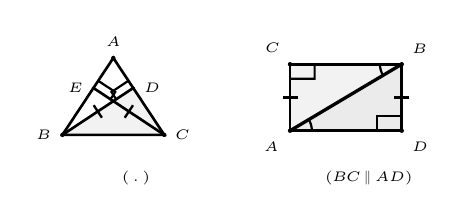
\begin{tikzpicture}[scale=0.66, every node/.style={font=\scriptsize, text=black}]
  % លំហាត់ទី១០ (ទំ.១៦៥)
  \begin{scope}[shift={(-2.15,0)}]
    \coordinate (A) at (0, 1.48);
    \coordinate (B) at (-0.98, 0);
    \coordinate (C) at (0.98, 0);
    \coordinate (D) at ($(A)!(B)!(C)$);
    \coordinate (E) at ($(A)!(C)!(B)$);
    \fill[gray!10] (B) -- (D) -- (C) -- cycle;
    \draw[black, line width=0.95pt] (A) -- (B) -- (C) -- cycle;
    \draw[black, line width=0.95pt, tk1] (B) -- (D);
    \draw[black, line width=0.95pt, tk1] (C) -- (E);
    \rightbox[0.24]{B}{D}{A}
    \rightbox[0.24]{C}{E}{A}
    \fill[black] (A) circle (1.2pt) node[above=0.5pt, font=\tiny] {$A$};
    \fill[black] (B) circle (1.2pt) node[left=0.5pt, font=\tiny] {$B$};
    \fill[black] (C) circle (1.2pt) node[right=0.5pt, font=\tiny] {$C$};
    \fill[black] (D) circle (1.0pt) node[right=0.5pt, font=\tiny] {$D$};
    \fill[black] (E) circle (1.0pt) node[left=0.5pt, font=\tiny] {$E$};
    \node[below=8pt, font=\tiny] at (0,-0.08) {លំហាត់ទី១០ (អ.ជ)};
  \end{scope}
  % លំហាត់ទី១២ (ទំ.១៦៥) + មុំឆ្លាស់ក្នុង
  \begin{scope}[shift={(1.25,0.08)}]
    \coordinate (A) at (0, 0);
    \coordinate (D) at (2.15, 0);
    \coordinate (C) at (0, 1.28);
    \coordinate (B) at (2.15, 1.28);
    \fill[gray!10] (A) -- (C) -- (B) -- cycle;
    \fill[gray!16] (A) -- (B) -- (D) -- cycle;
    \draw[black, line width=0.95pt] (C) -- (B) (A) -- (D);
    \draw[black, line width=0.95pt, tk1] (A) -- (C);
    \draw[black, line width=0.95pt, tk1] (B) -- (D);
    \draw[black, line width=1.20pt] (A) -- (B);
    \rightbox[0.22]{A}{C}{B}
    \rightbox[0.22]{B}{D}{A}
    \draw[black, line width=0.8pt] ($(B)+(-180:0.42)$) arc (-180:-149:0.42);
    \draw[black, line width=0.8pt] ($(A)+(0:0.42)$) arc (0:31:0.42);
    \fill[black] (A) circle (1.2pt) node[below left=0.5pt, font=\tiny] {$A$};
    \fill[black] (B) circle (1.2pt) node[above right=0.5pt, font=\tiny] {$B$};
    \fill[black] (C) circle (1.2pt) node[above left=0.5pt, font=\tiny] {$C$};
    \fill[black] (D) circle (1.2pt) node[below right=0.5pt, font=\tiny] {$D$};
    \node[below=8pt, font=\tiny] at (1.08,-0.16) {លំហាត់ទី១២ ($BC \parallel AD$)};
  \end{scope}
\end{tikzpicture}}

% ២. រំលឹកមេរៀនទាក់ទង៖ ចំណុចកណ្ដាល I, Δ⊥BC, ជ.ម.ជ (SAS) & ជ.ជ.ជ (SSS)
\newcommand{\figPrereqPB}{%
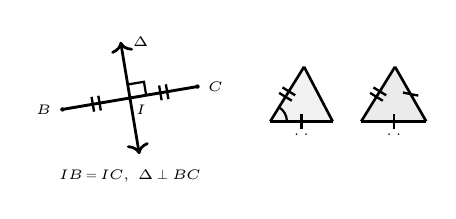
\begin{tikzpicture}[scale=0.66, every node/.style={font=\scriptsize, text=black}]
  % ឆ្វេង៖ I ចំណុចកណ្ដាល & Δ⊥BC
  \begin{scope}[shift={(-2.30,0.45)}]
    \coordinate (B) at (-1.30,-0.22);
    \coordinate (C) at (1.30,0.22);
    \coordinate (I) at (0,0);
    \coordinate (M) at (-0.18,1.08);
    \coordinate (N) at (0.18,-1.08);
    \draw[black, line width=1.05pt, tk2] (B) -- (I);
    \draw[black, line width=1.05pt, tk2] (I) -- (C);
    \draw[black, line width=1.0pt, <->] (N) -- (M) node[right=1pt, font=\tiny] {$\Delta$};
    \rightbox[0.24]{M}{I}{C}
    \fill[black] (B) circle (1.2pt) node[left=0.5pt, font=\tiny] {$B$};
    \fill[black] (C) circle (1.2pt) node[right=0.5pt, font=\tiny] {$C$};
    \fill[black] (I) circle (1.2pt) node[below right=-1pt, font=\tiny] {$I$};
    \node[below=10pt, font=\tiny] at (0,-0.65) {$IB=IC,\ \Delta\perp BC$};
  \end{scope}
  % ស្ដាំ៖ ជ.ម.ជ (SAS) vs ជ.ជ.ជ (SSS)
  \begin{scope}[shift={(1.50,0)}]
    \coordinate (P) at (-1.10,0);
    \coordinate (Q) at (0.10,0);
    \coordinate (R) at (-0.45,1.05);
    \fill[gray!10] (P) -- (Q) -- (R) -- cycle;
    \draw[black, line width=0.95pt, tk1] (P) -- (Q);
    \draw[black, line width=0.95pt, tk2] (P) -- (R);
    \draw[black, line width=0.95pt] (Q) -- (R);
    \draw[black, line width=0.8pt] (-0.78,0) arc (0:58:0.32);
    \node[font=\tiny] at (-0.50,-0.25) {ជ.ម.ជ};
    \coordinate (P2) at (0.65,0);
    \coordinate (Q2) at (1.90,0);
    \coordinate (R2) at (1.30,1.05);
    \fill[gray!16] (P2) -- (Q2) -- (R2) -- cycle;
    \draw[black, line width=0.95pt, tk1] (P2) -- (Q2);
    \draw[black, line width=0.95pt, tk2] (P2) -- (R2);
    \draw[black, line width=0.95pt, tkslash] (Q2) -- (R2);
    \node[font=\tiny] at (1.28,-0.25) {ជ.ជ.ជ};
    \node[below=10pt, font=\tiny] at (0.40,-0.20) {លក្ខខណ្ឌប៉ុនគ្នា};
  \end{scope}
\end{tikzpicture}}

% ៣. E1 Engage: ស្ថានីយបូមទឹកសូឡាភូមិ B & C (ប្រឡាយទឹកលិចត្រង់ I, ទ្រេត 12°)
\newcommand{\figEngagePB}{%
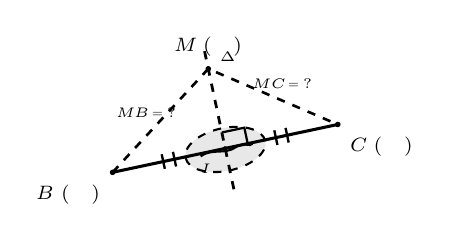
\begin{tikzpicture}[scale=0.68, every node/.style={font=\scriptsize, text=black}]
  \begin{scope}[rotate=12]
    \coordinate (B) at (-2.15,0);
    \coordinate (C) at (2.15,0);
    \coordinate (I) at (0,0);
    \coordinate (M) at (0,1.52);
    \coordinate (Dbot) at (0,-0.78);
    % ប្រឡាយទឹកលិចត្រង់ I
    \fill[gray!18] (0,-0.02) ellipse (0.76 and 0.40);
    \draw[black, line width=0.75pt, dashed] (0,-0.02) ellipse (0.76 and 0.40);
    \draw[black, line width=0.75pt] (-0.48,-0.05) .. controls (-0.24,0.06) and (-0.04,-0.12) .. (0.20,-0.02) .. controls (0.35,0.06) and (0.46,-0.08) .. (0.52,-0.02);
    \draw[black, line width=1.10pt, tk2] (B) -- (I);
    \draw[black, line width=1.10pt, tk2] (I) -- (C);
    \draw[black, line width=1.0pt, dashed] (Dbot) -- (0,1.88);
    \draw[black, line width=0.95pt, dashed] (B) -- (M) -- (C);
    \rightbox[0.20]{M}{I}{C}
    \fill[black] (B) circle (1.5pt) node[below left=1pt] {$B$ (ភូមិ)};
    \fill[black] (C) circle (1.5pt) node[below right=1pt] {$C$ (ភូមិ)};
    \fill[black] (I) circle (1.2pt) node[below left=2pt, font=\tiny] {$I$};
    \fill[black] (M) circle (1.5pt) node[above=1pt] {$M$ (សូឡា)};
    \node[font=\tiny, anchor=west] at (0.08,-0.76) {ប្រឡាយទឹកលិច};
    \node[font=\tiny] at (-1.30,0.96) {$MB=?$};
    \node[font=\tiny] at (1.30,0.96) {$MC=?$};
    \node[right=2pt, font=\tiny] at (0,1.76) {$\Delta$};
  \end{scope}
\end{tikzpicture}}

% ៤. E2 Act 1: បត់ក្រដាសបន្ទះទ្រេត 12° (BC = 6.0 cm, M=2.5 cm, N=3.5 cm)
\newcommand{\figExploreOnePB}{%
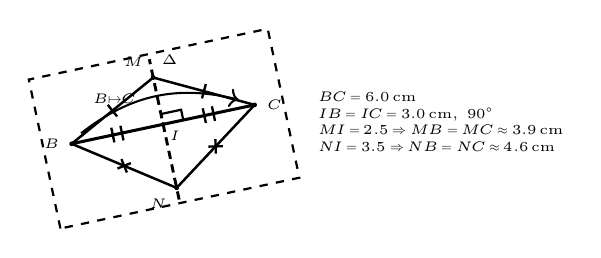
\begin{tikzpicture}[scale=0.66, every node/.style={font=\scriptsize, text=black}]
  \begin{scope}[rotate=12]
    \draw[black, line width=0.8pt, dashed] (-2.35,-1.55) rectangle (2.35,1.38);
    \coordinate (B) at (-1.80,0);
    \coordinate (C) at (1.80,0);
    \coordinate (I) at (0,0);
    \coordinate (M) at (0,0.92);
    \coordinate (N) at (0,-1.25);
    \draw[black, line width=1.10pt, tk2] (B) -- (I);
    \draw[black, line width=1.10pt, tk2] (I) -- (C);
    \draw[black, line width=1.05pt, densely dashed] (0,-1.48) -- (0,1.28) node[right=1pt, font=\tiny] {$\Delta$};
    \draw[black, line width=0.90pt, tk1] (M) -- (B);
    \draw[black, line width=0.90pt, tk1] (M) -- (C);
    \draw[black, line width=0.90pt, tkcross] (N) -- (B);
    \draw[black, line width=0.90pt, tkcross] (N) -- (C);
    \rightbox[0.22]{M}{I}{C}
    \draw[black, line width=0.75pt, ->, bend left=26] (-1.58,0.16) to (1.52,0.16);
    \node[font=\tiny] at (-0.98,0.72) {បត់ $B{\mapsto}C$};
    \fill[black] (B) circle (1.3pt) node[left=1pt, font=\tiny] {$B$};
    \fill[black] (C) circle (1.3pt) node[right=1pt, font=\tiny] {$C$};
    \fill[black] (I) circle (1.2pt) node[below right=-1pt, font=\tiny] {$I$};
    \fill[black] (M) circle (1.3pt) node[above left=0.5pt, font=\tiny] {$M$};
    \fill[black] (N) circle (1.3pt) node[below left=0.5pt, font=\tiny] {$N$};
  \end{scope}
  \node[right=6pt, align=left, font=\tiny] at (2.48,0.05) {%
    $BC=6.0\unit{cm}$\\
    $IB=IC=3.0\unit{cm},\ 90^\circ$\\
    $MI=2.5\Rightarrow MB=MC\approx 3.9\unit{cm}$\\
    $NI=3.5\Rightarrow NB=NC\approx 4.6\unit{cm}$%
  };
\end{tikzpicture}}

% ៥. E2 Act 2 Dual POE: Panel X (60°) + Panel Y (HB=2,HC=4) + POE 2B (r=4.5cm)
\newcommand{\figExploreTwoPB}{%
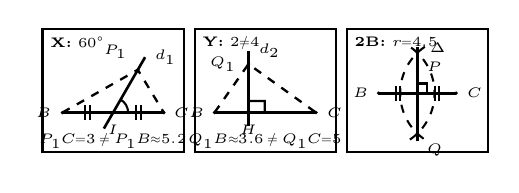
\begin{tikzpicture}[scale=0.56, every node/.style={font=\tiny, text=black}]
  % Panel X: Lock 1 តែម្ខាង (60°, IB=IC=3, P1I=3)
  \begin{scope}[shift={(0,0)}]
    \draw[black, line width=0.8pt] (-1.60,-0.82) rectangle (1.60,1.98);
    \node[anchor=north west, inner sep=2pt] at (-1.56,1.94) {\textbf{X:} $60^\circ$};
    \coordinate (B) at (-1.15,0.08);
    \coordinate (C) at (1.15,0.08);
    \coordinate (I) at (0,0.08);
    \coordinate (P1) at ($(I)+(60:1.12)$);
    \draw[black, line width=1.0pt, tk2] (B) -- (I);
    \draw[black, line width=1.0pt, tk2] (I) -- (C);
    \draw[black, line width=0.95pt] ($(I)+(-120:0.42)$) -- ($(I)+(60:1.45)$) node[right=0pt] {$d_1$};
    \draw[black, line width=0.85pt, dashed] (B) -- (P1) -- (C);
    \draw[black, line width=0.75pt] (0.34,0.08) arc (0:60:0.34);
    \fill[black] (B) circle (1.2pt) node[left=0.5pt] {$B$};
    \fill[black] (C) circle (1.2pt) node[right=0.5pt] {$C$};
    \fill[black] (I) circle (1.1pt) node[below=1pt] {$I$};
    \fill[black] (P1) circle (1.2pt) node[above left=0.5pt] {$P_1$};
    \node at (0,-0.56) {$P_1C{=}3\neq P_1B{\approx}5.2$};
  \end{scope}
  % Panel Y: Lock 2 តែម្ខាង (90°, HB=2, HC=4)
  \begin{scope}[shift={(3.45,0)}]
    \draw[black, line width=0.8pt] (-1.60,-0.82) rectangle (1.60,1.98);
    \node[anchor=north west, inner sep=2pt] at (-1.56,1.94) {\textbf{Y:} $2{\neq}4$};
    \coordinate (B) at (-1.15,0.08);
    \coordinate (C) at (1.15,0.08);
    \coordinate (H) at (-0.38,0.08);
    \coordinate (Q1) at (-0.38,1.18);
    \draw[black, line width=1.0pt] (B) -- (C);
    \draw[black, line width=0.95pt] (-0.38,-0.22) -- (-0.38,1.48) node[right=0pt] {$d_2$};
    \draw[black, line width=0.85pt, dashed] (B) -- (Q1) -- (C);
    \rightbox[0.24]{Q1}{H}{C}
    \fill[black] (B) circle (1.2pt) node[left=0.5pt] {$B$};
    \fill[black] (C) circle (1.2pt) node[right=0.5pt] {$C$};
    \fill[black] (H) circle (1.1pt) node[below=1pt] {$H$};
    \fill[black] (Q1) circle (1.2pt) node[left=1pt] {$Q_1$};
    \node at (0,-0.56) {$Q_1B{\approx}3.6\neq Q_1C{=}5$};
  \end{scope}
  % POE 2B: ធ្នូដែកឈាន r=4.5 cm កាត់ P, Q
  \begin{scope}[shift={(6.90,0)}]
    \draw[black, line width=0.8pt] (-1.60,-0.82) rectangle (1.60,1.98);
    \node[anchor=north west, inner sep=2pt] at (-1.56,1.94) {\textbf{2B:} $r{=}4.5$};
    \coordinate (B) at (-0.88,0.52);
    \coordinate (C) at (0.88,0.52);
    \coordinate (I) at (0,0.52);
    \coordinate (P) at (0,1.44);
    \coordinate (Q) at (0,-0.40);
    \draw[black, line width=1.0pt, tk2] (B) -- (I);
    \draw[black, line width=1.0pt, tk2] (I) -- (C);
    \draw[black, line width=0.75pt, dashed] ($(B)+(-56:1.27)$) arc (-56:56:1.27);
    \draw[black, line width=0.75pt, dashed] ($(C)+(124:1.27)$) arc (124:236:1.27);
    \draw[black, line width=1.05pt] (0,-0.56) -- (0,1.56) node[right=1pt] {$\Delta$};
    \rightbox[0.24]{P}{I}{C}
    \fill[black] (B) circle (1.2pt) node[left=0.5pt] {$B$};
    \fill[black] (C) circle (1.2pt) node[right=0.5pt] {$C$};
    \fill[black] (P) circle (1.2pt) node[below right=0pt] {$P$};
    \fill[black] (Q) circle (1.2pt) node[below right=0pt] {$Q$};
  \end{scope}
\end{tikzpicture}}

% ៦. E3 Explain: រូបសៀវភៅគោល ទំ.១៥៦ (BC ឈរត្រង់ C លើ B ក្រោម, Δ ដេក M ឆ្វេង N ស្ដាំ)
\newcommand{\figExplainPB}{%
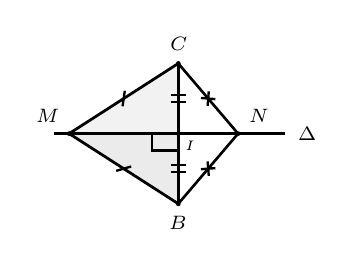
\begin{tikzpicture}[scale=0.66, every node/.style={font=\scriptsize, text=black}]
  \coordinate (C) at (0, 1.35);
  \coordinate (B) at (0, -1.35);
  \coordinate (I) at (0, 0);
  \coordinate (M) at (-2.10, 0);
  \coordinate (N) at (1.15, 0);
  \fill[gray!10] (M) -- (C) -- (I) -- cycle;
  \fill[gray!16] (M) -- (I) -- (B) -- cycle;
  \draw[black, line width=1.05pt, tk2] (C) -- (I);
  \draw[black, line width=1.05pt, tk2] (I) -- (B);
  \draw[black, line width=1.05pt] (-2.40,0) -- (2.05,0) node[right=1pt] {$\Delta$};
  \draw[black, line width=1.0pt, tkslash] (M) -- (C);
  \draw[black, line width=1.0pt, tkslash] (M) -- (B);
  \draw[black, line width=0.95pt, tkcross] (N) -- (C);
  \draw[black, line width=0.95pt, tkcross] (N) -- (B);
  \rightbox[0.24]{M}{I}{B}
  \fill[black] (C) circle (1.3pt) node[above=1pt] {$C$};
  \fill[black] (B) circle (1.3pt) node[below=1pt] {$B$};
  \fill[black] (I) circle (1.2pt) node[below right=-1pt, font=\tiny] {$I$};
  \fill[black] (M) circle (1.3pt) node[above left=0.5pt] {$M$};
  \fill[black] (N) circle (1.3pt) node[above right=0.5pt] {$N$};
\end{tikzpicture}}

% ៧. E3 Explain Inset: ប្រៀបធៀប ពុះមុំ (កែងជ្រុង) vs មេដ្យាទ័រ (ស្មើចុង)
\newcommand{\figLocusContrastPB}{%
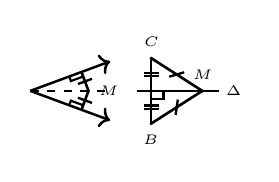
\begin{tikzpicture}[scale=0.52, every node/.style={font=\tiny, text=black}]
  % ឆ្វេង៖ ពុះមុំ (កែងជ្រុង)
  \begin{scope}[shift={(0,0.95)}]
    \coordinate (O) at (0,0);
    \coordinate (X) at (1.95, 0.72);
    \coordinate (Y) at (1.95, -0.72);
    \coordinate (M) at (1.42, 0);
    \coordinate (A) at ($(O)!(M)!(X)$);
    \coordinate (B) at ($(O)!(M)!(Y)$);
    \draw[black, line width=0.9pt, ->] (O) -- (X);
    \draw[black, line width=0.9pt, ->] (O) -- (Y);
    \draw[black, line width=0.85pt, dashed] (O) -- (1.95,0);
    \draw[black, line width=0.95pt, tk1] (M) -- (A);
    \draw[black, line width=0.95pt, tk1] (M) -- (B);
    \rightbox[0.24]{M}{A}{O}
    \rightbox[0.24]{M}{B}{O}
    \fill[black] (M) circle (1.1pt) node[right=0.5pt] {$M$};
    \node[below=2pt] at (0.95,-0.78) {ពុះមុំ៖ កែងជ្រុង};
  \end{scope}
  % ស្ដាំ៖ មេដ្យាទ័រ (ស្មើចុង)
  \begin{scope}[shift={(2.95,0.95)}]
    \coordinate (B) at (0,-0.80);
    \coordinate (C) at (0,0.80);
    \coordinate (I) at (0,0);
    \coordinate (M) at (1.25,0);
    \draw[black, line width=0.95pt, tk2] (B) -- (I);
    \draw[black, line width=0.95pt, tk2] (I) -- (C);
    \draw[black, line width=0.9pt] (-0.35,0) -- (1.65,0) node[right=-1pt] {$\Delta$};
    \draw[black, line width=0.95pt, tkslash] (M) -- (B);
    \draw[black, line width=0.95pt, tkslash] (M) -- (C);
    \rightbox[0.24]{M}{I}{B}
    \fill[black] (B) circle (1.1pt) node[below=0.5pt] {$B$};
    \fill[black] (C) circle (1.1pt) node[above=0.5pt] {$C$};
    \fill[black] (M) circle (1.1pt) node[above=0.5pt] {$M$};
    \node[below=2pt] at (0.75,-0.80) {មេដ្យាទ័រ៖ ស្មើចុង};
  \end{scope}
\end{tikzpicture}}

% ៨. E4 Elaborate: លំហាត់គំរូ ទ្រឹស្ដីបទច្រាស (MI ជំនួយ [tracing]) & ២ ចំណុច vs ១ ចំណុច
\newcommand{\figModelPB}{%
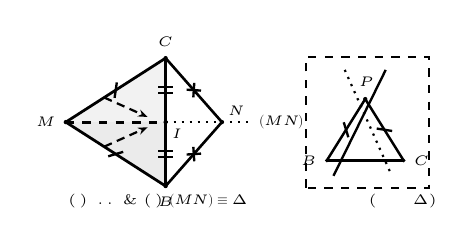
\begin{tikzpicture}[scale=0.65, every node/.style={font=\scriptsize, text=black}]
  % ឆ្វេង៖ សម្រាយច្រាស ជ.ជ.ជ + 2 ចំណុច (MN) ≡ Δ
  \begin{scope}[shift={(0,0)}]
    \coordinate (C) at (0,1.25);
    \coordinate (B) at (0,-1.25);
    \coordinate (I) at (0,0);
    \coordinate (M) at (-1.95,0);
    \coordinate (N) at (1.10,0);
    \fill[gray!10] (M) -- (C) -- (I) -- cycle;
    \fill[gray!16] (M) -- (I) -- (B) -- cycle;
    \draw[black, line width=1.0pt, tk2] (C) -- (I);
    \draw[black, line width=1.0pt, tk2] (I) -- (B);
    \draw[black, line width=1.05pt, dashed] (M) -- (I);
    \draw[black, line width=0.9pt, dotted] (I) -- (1.60,0) node[right=0.5pt, font=\tiny] {$(MN)$};
    \draw[black, line width=1.0pt, tkslash] (M) -- (C);
    \draw[black, line width=1.0pt, tkslash] (M) -- (B);
    \draw[black, line width=0.95pt, tkcross] (N) -- (C);
    \draw[black, line width=0.95pt, tkcross] (N) -- (B);
    \draw[hypArrow] ($(M)+(0.75,0.48)$) -- ($(I)+(-0.35,0.10)$);
    \draw[hypArrow] ($(M)+(0.75,-0.48)$) -- ($(I)+(-0.35,-0.10)$);
    \fill[black] (C) circle (1.2pt) node[above=0.5pt, font=\tiny] {$C$};
    \fill[black] (B) circle (1.2pt) node[below=0.5pt, font=\tiny] {$B$};
    \fill[black] (I) circle (1.2pt) node[below right=-1pt, font=\tiny] {$I$};
    \fill[black] (M) circle (1.2pt) node[left=0.5pt, font=\tiny] {$M$};
    \fill[black] (N) circle (1.2pt) node[above right=-1pt, font=\tiny] {$N$};
    \node[font=\tiny] at (-0.15,-1.54) {(ក) ជ.ជ.ជ \& (ខ) $(MN)\equiv\Delta$};
  \end{scope}
  % ស្ដាំ៖ អន្ទាក់ ១ ចំណុច (P ស្មើចម្ងាយ ប៉ុន្តែបន្ទាត់ទ្រេតជាច្រើន)
  \begin{scope}[shift={(3.80,0)}]
    \draw[black, line width=0.75pt, dashed] (-1.05,-1.28) rectangle (1.35,1.28);
    \coordinate (B) at (-0.65,-0.75);
    \coordinate (C) at (0.85,-0.75);
    \coordinate (P) at (0.10,0.45);
    \draw[black, line width=1.0pt] (B) -- (C);
    \draw[black, line width=0.9pt, tkslash] (P) -- (B);
    \draw[black, line width=0.9pt, tkslash] (P) -- (C);
    \draw[black, line width=0.85pt] (-0.52,-1.05) -- (0.50,1.02);
    \draw[black, line width=0.8pt, dotted] (-0.30,1.02) -- (0.62,-1.05);
    \fill[black] (B) circle (1.1pt) node[left=0.5pt, font=\tiny] {$B$};
    \fill[black] (C) circle (1.1pt) node[right=0.5pt, font=\tiny] {$C$};
    \fill[black] (P) circle (1.2pt) node[above=1pt, font=\tiny] {$P$};
    \node[font=\tiny] at (0.15,-1.54) {អន្ទាក់ ១ ចំណុច (មិនកំណត់ $\Delta$)};
  \end{scope}
\end{tikzpicture}}

% ៩. E5 Evaluate: ប្រតិបត្តិ (ស្ថានីយបូមទឹកសូឡា BC=8 cm, M លើ Δ, N មាន NB=NC=6 cm)
\newcommand{\figPracticePB}{%
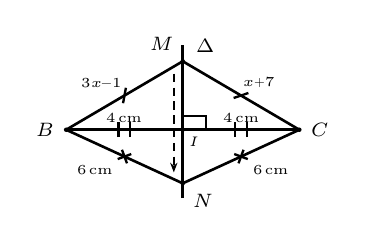
\begin{tikzpicture}[scale=0.63, every node/.style={font=\scriptsize, text=black}]
  \coordinate (B) at (-2.35,0);
  \coordinate (C) at (2.35,0);
  \coordinate (I) at (0,0);
  \coordinate (M) at (0,1.38);
  \coordinate (N) at (0,-1.08);
  \draw[black, line width=1.10pt, tk2] (B) -- (I);
  \draw[black, line width=1.10pt, tk2] (I) -- (C);
  \draw[black, line width=1.05pt] (0,-1.38) -- (0,1.70) node[right=1pt] {$\Delta$};
  \draw[black, line width=0.95pt, tkslash] (M) -- (B);
  \draw[black, line width=0.95pt, tkslash] (M) -- (C);
  \draw[black, line width=0.95pt, tkcross] (N) -- (B);
  \draw[black, line width=0.95pt, tkcross] (N) -- (C);
  \rightbox[0.20]{M}{I}{C}
  \draw[hypArrow] ($(M)+(-0.18,-0.25)$) -- ($(N)+(-0.18,0.22)$);
  \node[font=\tiny, above left=-1pt] at (-1.08,0.70) {$3x{-}1$};
  \node[font=\tiny, above right=-1pt] at (1.08,0.70) {$x{+}7$};
  \node[font=\tiny, below left=0pt] at (-1.22,-0.52) {$6\unit{cm}$};
  \node[font=\tiny, below right=0pt] at (1.22,-0.52) {$6\unit{cm}$};
  \node[font=\tiny] at (-1.18,0.24) {$4\unit{cm}$};
  \node[font=\tiny] at (1.18,0.24) {$4\unit{cm}$};
  \fill[black] (B) circle (1.3pt) node[left=1pt] {$B$};
  \fill[black] (C) circle (1.3pt) node[right=1pt] {$C$};
  \fill[black] (I) circle (1.2pt) node[below right=-1pt, font=\tiny] {$I$};
  \fill[black] (M) circle (1.3pt) node[above left=0.5pt] {$M$};
  \fill[black] (N) circle (1.3pt) node[below right=0.5pt] {$N$};
\end{tikzpicture}}

% ១០. E5 Evaluate: កាតត្រួតពិនិត្យ A–D
\newcommand{\figExitCardsPB}{%
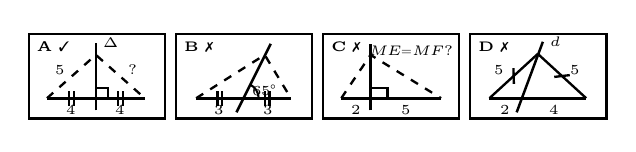
\begin{tikzpicture}[scale=0.64, every node/.style={font=\tiny, text=black}]
  % កាត A: Δ⊥AB ត្រង់ I, IA=IB=4, MA=5 => MB=5 ✓
  \begin{scope}[shift={(0,0)}]
    \draw[black, line width=0.85pt] (0,0) rectangle (2.70,1.68);
    \node[anchor=north west, inner sep=2pt] at (0.04,1.64) {\textbf{A} \ding{51}};
    \coordinate (A) at (0.36,0.40);
    \coordinate (B) at (2.30,0.40);
    \coordinate (I) at (1.33,0.40);
    \coordinate (M) at (1.33,1.26);
    \draw[black, line width=0.95pt, tk2] (A) -- (I);
    \draw[black, line width=0.95pt, tk2] (I) -- (B);
    \draw[black, line width=0.9pt] (1.33,0.16) -- (1.33,1.50) node[right=-1pt] {$\Delta$};
    \draw[black, line width=0.85pt, dashed] (A) -- (M) -- (B);
    \rightbox[0.24]{M}{I}{B}
    \node at (0.62,0.96) {$5$};
    \node at (2.06,0.96) {$?$};
    \node at (0.85,0.16) {$4$};
    \node at (1.82,0.16) {$4$};
  \end{scope}
  % កាត B: មេដ្យានទ្រេត 65° ✗
  \begin{scope}[shift={(2.92,0)}]
    \draw[black, line width=0.85pt] (0,0) rectangle (2.70,1.68);
    \node[anchor=north west, inner sep=2pt] at (0.04,1.64) {\textbf{B} \ding{55}};
    \coordinate (C) at (0.40,0.40);
    \coordinate (D) at (2.28,0.40);
    \coordinate (I) at (1.34,0.40);
    \coordinate (M) at (1.76,1.26);
    \draw[black, line width=0.95pt, tk2] (C) -- (I);
    \draw[black, line width=0.95pt, tk2] (I) -- (D);
    \draw[black, line width=0.9pt] (1.20,0.12) -- (1.88,1.48);
    \draw[black, line width=0.85pt, dashed] (C) -- (M) -- (D);
    \draw[black, line width=0.75pt] (1.64,0.40) arc (0:65:0.30);
    \node at (1.76,0.55) {$65^\circ$};
    \node at (0.86,0.16) {$3$};
    \node at (1.82,0.16) {$3$};
  \end{scope}
  % កាត C: កែងខុសចំណុចកណ្ដាល HE=2, HF=5 ✗
  \begin{scope}[shift={(5.84,0)}]
    \draw[black, line width=0.85pt] (0,0) rectangle (2.70,1.68);
    \node[anchor=north west, inner sep=2pt] at (0.04,1.64) {\textbf{C} \ding{55}};
    \coordinate (E) at (0.36,0.40);
    \coordinate (F) at (2.34,0.40);
    \coordinate (H) at (0.94,0.40);
    \coordinate (M) at (0.94,1.26);
    \draw[black, line width=0.95pt] (E) -- (F);
    \draw[black, line width=0.9pt] (0.94,0.16) -- (0.94,1.48);
    \draw[black, line width=0.85pt, dashed] (E) -- (M) -- (F);
    \rightbox[0.24]{M}{H}{F}
    \node at (0.65,0.16) {$2$};
    \node at (1.65,0.16) {$5$};
    \node at (1.75,1.34) {$ME{=}MF?$};
  \end{scope}
  % កាត D: អន្ទាក់ ១ ចំណុច PG=PH=5, d ទ្រេតកាត់ K (2 vs 4) ✗
  \begin{scope}[shift={(8.76,0)}]
    \draw[black, line width=0.85pt] (0,0) rectangle (2.70,1.68);
    \node[anchor=north west, inner sep=2pt] at (0.04,1.64) {\textbf{D} \ding{55}};
    \coordinate (G) at (0.38,0.40);
    \coordinate (H) at (2.30,0.40);
    \coordinate (K) at (1.02,0.40);
    \coordinate (P) at (1.34,1.28);
    \draw[black, line width=0.95pt] (G) -- (H);
    \draw[black, line width=0.85pt, tkslash] (P) -- (G);
    \draw[black, line width=0.85pt, tkslash] (P) -- (H);
    \draw[black, line width=0.9pt] (0.92,0.12) -- (1.44,1.52) node[right=-1pt] {$d$};
    \node at (0.70,0.16) {$2$};
    \node at (1.66,0.16) {$4$};
    \node at (0.58,0.96) {$5$};
    \node at (2.08,0.96) {$5$};
  \end{scope}
\end{tikzpicture}}

% ១១. ជំហានទី៥ កិច្ចការផ្ទះ៖ លំហាត់ទី១, ទី៣ (+ បំបែក) និង ទី៥ (+ (ខ) Δ⊥RS) (ទំ.១៦៤)
\newcommand{\figHWnewPB}{%
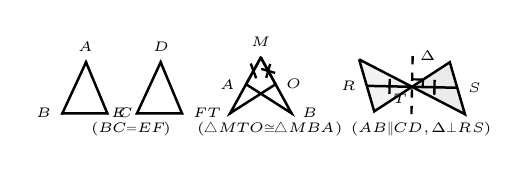
\begin{tikzpicture}[scale=0.60, every node/.style={font=\tiny, text=black}]
  % លំហាត់ទី១៖ △ABC ≅ △DEF
  \begin{scope}[shift={(-4.35,0)}]
    \coordinate (B) at (0,0);
    \coordinate (C) at (0.95,0);
    \coordinate (A) at (0.50,1.08);
    \draw[black, line width=0.9pt] (A) -- (B) -- (C) -- cycle;
    \fill[black] (A) circle (1.0pt) node[above=0.5pt] {$A$};
    \fill[black] (B) circle (1.0pt) node[left=0.5pt] {$B$};
    \fill[black] (C) circle (1.0pt) node[right=0.5pt] {$C$};
    \coordinate (E) at (1.58,0);
    \coordinate (F) at (2.53,0);
    \coordinate (D) at (2.08,1.08);
    \draw[black, line width=0.9pt] (D) -- (E) -- (F) -- cycle;
    \fill[black] (D) circle (1.0pt) node[above=0.5pt] {$D$};
    \fill[black] (E) circle (1.0pt) node[left=0.5pt] {$E$};
    \fill[black] (F) circle (1.0pt) node[right=0.5pt] {$F$};
    \node at (1.26,-0.34) {ទី១ ($BC{=}EF$)};
  \end{scope}
  % លំហាត់ទី៣៖ រូបត្រួត V + បំបែក
  \begin{scope}[shift={(-0.15,0)}]
    \coordinate (M) at (0,1.18);
    \coordinate (T) at (-0.65,0);
    \coordinate (B) at (0.65,0);
    \coordinate (A) at ($(M)!0.48!(T)$);
    \coordinate (O) at ($(M)!0.48!(B)$);
    \draw[black, line width=0.9pt] (M) -- (T) -- (O) (M) -- (B) -- (A);
    \draw[black, line width=0.85pt, tkslash] (M) -- (A);
    \draw[black, line width=0.85pt, tkcross] (M) -- (O);
    \fill[black] (M) circle (1.0pt) node[above=0.5pt] {$M$};
    \fill[black] (A) circle (0.9pt) node[left=0.5pt] {$A$};
    \fill[black] (O) circle (0.9pt) node[right=0.5pt] {$O$};
    \fill[black] (T) circle (0.9pt) node[left=0.5pt] {$T$};
    \fill[black] (B) circle (0.9pt) node[right=0.5pt] {$B$};
    \node at (0,-0.34) {ទី៣ ($\tri{MTO}{\cg}\tri{MBA}$)};
  \end{scope}
  % លំហាត់ទី៥៖ មេអំបៅ AB∥CD, TR=TS + Δ⊥RS
  \begin{scope}[shift={(3.05,0.56)}]
    \coordinate (T) at (0,0);
    \coordinate (A) at (-1.12,0.58);
    \coordinate (B) at (-0.80,-0.52);
    \coordinate (C) at (0.80,0.52);
    \coordinate (D) at (1.12,-0.58);
    \coordinate (R) at (-0.95,0.02);
    \coordinate (S) at (0.95,-0.02);
    \fill[gray!10] (A) -- (B) -- (T) -- cycle;
    \fill[gray!16] (C) -- (D) -- (T) -- cycle;
    \draw[black, line width=0.9pt] (A) -- (B) -- (C) -- (D) -- (A);
    \draw[black, line width=0.9pt, tk1] (R) -- (T);
    \draw[black, line width=0.9pt, tk1] (T) -- (S);
    \coordinate (Dbot) at (-0.012,-0.58);
    \coordinate (Dtop) at (0.014,0.66);
    \draw[black, line width=0.85pt, dashed] (Dbot) -- (Dtop) node[right=-1pt] {$\Delta$};
    \rightbox[0.24]{Dtop}{T}{S}
    \fill[black] (T) circle (1.0pt) node[below left=-1pt] {$T$};
    \fill[black] (R) circle (0.9pt) node[left=0.5pt] {$R$};
    \fill[black] (S) circle (0.9pt) node[right=0.5pt] {$S$};
    \node at (0,-0.90) {ទី៥ ($AB{\parallel}CD, \Delta{\perp}RS$)};
  \end{scope}
\end{tikzpicture}}

% ============================================================================
% ចាប់ផ្ដើមឯកសារ (Document Body)
% ============================================================================
\begin{document}
\fontsize{9.5pt}{14.0pt}\selectfont

% -------------------- ក្បាលកិច្ចតែងការ (Header) --------------------
\begin{center}
  {\muol\fontsize{11pt}{16pt}\selectfont ព្រះរាជាណាចក្រកម្ពុជា}\\[2pt]
  {\muol\fontsize{10pt}{15pt}\selectfont ជាតិ សាសនា ព្រះមហាក្សត្រ}\\[1pt]
  \khmflourish
\end{center}

\vspace{-15pt}
{\muol\fontsize{9.5pt}{13.2pt}\selectfont
មន្ទីរអប់រំ យុវជន និងកីឡា ខេត្តកំពង់ធំ\\
ការិយាល័យអប់រំ យុវជន និងកីឡា ស្រុកកំពង់ស្វាយ\\
អនុវិទ្យាល័យព្រះក្រសាំង}

\vspace{2pt}
\begin{center}
  {\muol\fontsize{10pt}{15pt}\selectfont កិច្ចតែងការបង្រៀន}
\end{center}
\vspace{1pt}

% -------------------- ព័ត៌មានទូទៅ (Metadata) --------------------
{\renewcommand{\arraystretch}{1.05}
\hspace*{4.05cm}%
\begin{tabular}{@{}l l l@{}}
  - \hspace{0.35cm} មុខវិជ្ជា & : & គណិតវិទ្យា ថ្នាក់ទី៨ \\
  - \hspace{0.35cm} ចំណងជើងមេរៀន & : & មេរៀនទី១២ ការប្រៀបធៀបត្រីកោណ \\
  - \hspace{0.35cm} ចំណងជើងរង & : & ២. មេដ្យាទ័រនៃអង្កត់និងត្រីកោណសមបាទ \\
  & & ២.១ លក្ខណៈមេដ្យាទ័រនៃអង្កត់ \\
  - \hspace{0.35cm} រយៈពេល & : & ១ ម៉ោងសិក្សា (៥០នាទី) \\
  - \hspace{0.35cm} បង្រៀនដោយ & : & ហុក ប៊ុនថែន \\
  - \hspace{0.35cm} កាលបរិច្ឆេទ & : & ថ្ងៃអង្គារ ទី១ ខែធ្នូ ឆ្នាំ២០២៦ \\
\end{tabular}

\vspace{2pt}

% -------------------- I. វត្ថុបំណង --------------------
\textbf{I.} {\muol វត្ថុបំណង}\\[2pt]
\hspace*{0.55cm}%
\begin{tabular}{@{}l l l@{}}
  \wcirc \hspace{0.25cm} វិជ្ជាសម្បទា & : & សិស្សកំណត់បានលក្ខខណ្ឌសោភ្លោះនៃមេដ្យាទ័រ ($IB=IC$ និង $\Delta\perp BC$) តាមបត់ក្រដាស $6\text{ cm}$ \\
  & & និង Dual POE ដែកឈាន ព្រមទាំងស្រាយបញ្ជាក់ទ្រឹស្ដីបទផ្ទាល់ (ជ.ម.ជ) និងច្រាស (ជ.ជ.ជ) ។ \\
  \wcirc \hspace{0.25cm} បំណិនសម្បទា & : & សិស្សបត់ $B\mapsto C$ សង់ធ្នូដែកឈាន $r=4.5\text{ cm}$ គូស \textbf{[tracing]} ប្រើធនាគារ \cnum{1}--\cnum{5} \\
  & & រក $x=4, MB=MC=11\text{ cm}$ និងបញ្ជាក់ ២ ចំណុច $(MN)\equiv\Delta$ ដោយមិនបាច់វាស់ $I$ ។ \\
  \wcirc \hspace{0.25cm} ចរិយាសម្បទា & : & សិស្សសហការជា «ក្រុមគណៈកម្មការវាស់ស្ទង់ទីតាំងស្មើចម្ងាយ» ផ្ទៀងសោភ្លោះមុនសន្និដ្ឋាន \\
  & & និងចៀសវាងអន្ទាក់ ១ ចំណុច ព្រមទាំងញែកមេដ្យាទ័រ (ស្មើចុង) ពីពុះមុំ (កែងជ្រុង) ច្បាស់លាស់ ។ \\
\end{tabular}

\vspace{2pt}

% -------------------- II. សម្ភារៈឧបទេស --------------------
\textbf{II.} {\muol សម្ភារៈឧបទេស}\\[2pt]
\hspace*{0.55cm}$\bullet$ \hspace{0.35cm} សៀវភៅគោលទី៨ (ទំ.១៥៦, ១៦៤) បន្ទាត់ក្រិត ១:១ ដែកឈាន រ៉ាព័រទ័រ កន្ត្រៃ កញ្ចប់ ១:១ (ទំព័រ ១) កាត E4--E5 (ទំព័រ ២--៣) ផ្ទាំង \cnum{1}--\cnum{5} (ទំព័រ ៤) កាត A--D (ទំព័រ ៥) និងប័ណ្ណកិច្ចការផ្ទះ (ទំព័រ ៦)

\vspace{2pt}

% -------------------- III. វិធីសាស្រ្តបង្រៀន --------------------
\textbf{III.} {\muol វិធីសាស្រ្តបង្រៀន}\\[2pt]
\hspace*{0.55cm}%
\begin{tabular}{@{}l l l@{}}
  $\bullet$ \hspace{0.35cm} គោលវិធី & : \hspace{0.7cm} & សិស្សមជ្ឈមណ្ឌល \\
  $\bullet$ \hspace{0.35cm} យុទ្ធវិធីបង្រៀន & : & ស្ថាបនានិយម គម្រូ 5Es (បត់ក្រដាស ១:១ Dual POE ដែកឈាន សោភ្លោះ \textbf{[tracing]} \& ៣ តួនាទី) \\
\end{tabular}
}

\vspace{2pt}

% -------------------- IV. ដំណើរការបង្រៀន --------------------
\textbf{IV.} {\muol ដំណើរការបង្រៀន}

\vspace{-3pt}

% ============================================================================
% តារាងដំណើរការបង្រៀន (Modular Multi-Row 3-Column Table – 50 នាទី)
% ============================================================================
\renewcommand{\arraystretch}{1.17}
\begin{longtable}{|L{5.50cm}|L{7.90cm}|L{4.80cm}|}
\hline
\rowcolor{headgray}
\multicolumn{1}{|c|}{\muol សកម្មភាពគ្រូ} &
\multicolumn{1}{c|}{\muol ខ្លឹមសារមេរៀន} &
\multicolumn{1}{c|}{\muol សកម្មភាពសិស្ស} \\
\hline
\endfirsthead

\hline
\endhead

\hline
\endfoot

\hline
\endlastfoot

% ==================== ជំហានទី១ (2min) ====================
\stepheader{ជំហានទី១ \enbf{(}រដ្ឋបាលថ្នាក់\enbf{)}}
- ពិនិត្យអវត្តមាន និងអនាម័យថ្នាក់រៀន \newline
- ចាត់ក្រុម ៣ នាក់ («ក្រុមគណៈកម្មការវាស់ស្ទង់ទីតាំងស្មើចម្ងាយ») និងចែកកញ្ចប់ ១:១ (ទំព័រ ១) ដាក់ផ្កាប់លើតុ
&
\hspace*{0.3cm}- រដ្ឋបាលថ្នាក់ \newline
\hspace*{0.3cm}- អនាម័យ និងសណ្ដាប់ធ្នាប់ថ្នាក់រៀន \newline
\hspace*{0.3cm}- ត្រៀមក្រុមគណៈកម្មការវាស់ស្ទង់ទីតាំងស្មើចម្ងាយ
&
- រាយការណ៍អវត្តមាន \newline
- អង្គុយតាមក្រុម ៣ នាក់ \\
\hline

% ==================== ជំហានទី២ (9min: HW 3m + Prereq 3m + E1 3m) ====================
\stepheader{ជំហានទី២ \enbf{(}កិច្ចការផ្ទះ \enbf{+} ទំនាក់ទំនងមេរៀនថ្មី\enbf{)}}
% --- ២.១ កំណែកិច្ចការផ្ទះ ---
- ពិនិត្យកិច្ចការផ្ទះ (លំហាត់ទី១០ និងទី១២ ទំ.១៦៥) \newline
\ditem \textbf{សំណួរបញ្ឆោត} ៖ «ហេតុអ្វីក្នុងលំហាត់ទី១២ ពី $\ang{CBA}=\ang{DAB}$ យើងទាញបាន $BC \parallel AD$?» \newline
\timenote{ចំណាយពេលឱ្យតិចបំផុតកុំឱ្យលើស 3min}
&
\centerline{\redsub{កំណែកិច្ចការផ្ទះ (លំហាត់ទី១០ \& ទី១២ ទំ.១៦៥)}}
\cfig{\figHWoldPB}
- ទី១០៖ $\tri{BDC}\cg\tri{CEB}$ (អ.ជ៖ $90^\circ$, អ៊ីប៉ូរួម $BC$, $BD=CE$) $\Rightarrow \ang{ABC}=\ang{ACB}$ \newline
- ទី១២៖ $\tri{ACB}\cg\tri{BDA}$ (អ.ជ៖ $AB$ រួម, $AC=BD$) $\Rightarrow \ang{CBA}=\ang{DAB}$ \graybox{មុំឆ្លាស់ក្នុងស្មើគ្នា $\Rightarrow BC\parallel AD$}
&
- ផ្ទៀង និងឆ្លើយ៖ «ព្រោះ $\ang{CBA}$ និង $\ang{DAB}$ ជាមុំឆ្លាស់ក្នុងស្មើគ្នា ទើប $BC \parallel AD$!» \\[-2pt]

% --- ២.២ រំលឹកមេរៀនទាក់ទង (3min) ---
\ditem \textbf{រំលឹករហ័ស (3min)} ៖ \newline
+ តើចំណុចកណ្ដាល $I$ នៃ $BC$ និងបន្ទាត់ $\Delta\perp BC$ ត្រង់ $I$ ផ្ដល់លក្ខណៈអ្វីខ្លះ? \newline
+ រំលឹកលក្ខខណ្ឌប៉ុនគ្នា ជ.ម.ជ (SAS) និង ជ.ជ.ជ (SSS) \newline
\timenote{សរុបកុំឱ្យលើស 3min}
&
\centerline{\redsub{រំលឹកមេរៀនទាក់ទងមេរៀនថ្មី}}
\cfig{\figPrereqPB}
- $I$ ចំណុចកណ្ដាល $BC \Rightarrow IB=IC$ \quad $\vert$ \quad $\Delta\perp BC$ ត្រង់ $I \Rightarrow \ang{MIB}=\ang{MIC}=90^\circ$ \newline
- លក្ខខណ្ឌ ជ.ម.ជ (SAS) \& ជ.ជ.ជ (SSS)
&
- ឆ្លើយ៖ «$IB=IC$ និងមុំត្រង់ $I$ ស្មើ $90^\circ$; ប្រើ ជ.ម.ជ និង ជ.ជ.ជ!» \\[-2pt]

% --- ២.៣ E1 Engage: បញ្ហាដាក់ស្ថានីយបូមទឹកសូឡា ---
\fiveE{E1 - Engage (3min)} \newline
\ditem \textbf{បញ្ហាដាក់ស្ថានីយបូមទឹកសូឡាស្មើចម្ងាយពីភូមិ $B$ និងភូមិ $C$} ៖ ភូមិ $B, C$ ចង់ដាក់ម៉ាស៊ីនបូមទឹក $M$ ឱ្យ $MB=MC$ ប៉ុន្តែចំណុចកណ្ដាល $I$ ស្ថិតក្នុង \textbf{ប្រឡាយទឹកលិច} ។ តើដាក់ $M$ នៅលើទីទួលខ្ពស់ខាងណាបានខ្លះ?
&
\centerline{\redsub{ស្ថានភាពពិត៖ ស្ថានីយបូមទឹកសូឡាភូមិ $B$ និងភូមិ $C$}}
\cfig{\figEngagePB}
\hspace*{0.1cm}\textbf{ចម្ងល់} ៖ ចៀសពីប្រឡាយទឹកលិចត្រង់ $I$ តើទីតាំង $M$ ណាខ្លះរក្សា $MB=MC$?
&
- ទស្សន៍ទាយថាអាចប្ដូរ $M$ ទៅលើខ្សែកែងលើដីគោកខាងលើ/ក្រោម $I$ \\
\hline

% ==================== ជំហានទី៣ (17min: E2 11m + E3 6m) ====================
\stepheader{ជំហានទី៣ \enbf{(}ខ្លឹមសារមេរៀនថ្មី\enbf{)}}
% --- ៣.១ ចំណងជើង & E2 Act 1 (6min) ---
- សរសេរចំណងជើងមេរៀនលើក្ដារខៀន \newline
\fiveE{E2 - Explore (11min)} \newline
\ditem \textbf{សកម្មភាព ១៖ បត់ក្រដាស $BC=6.0\text{ cm}$ (6min)} \newline
\hspace*{0.1cm}+ ផ្ទៀងក្រិត $5.0\text{ cm}$ លើទំព័រ ១ (១:១) រួចកាត់បន្ទះ ១ ($BC=6.0\text{ cm}$ ទ្រេត $12^\circ$) បត់ $B\mapsto C$ បង្កើតផ្នត់ $\Delta$ កាត់ $I$ \newline
\hspace*{0.1cm}+ វាស់ចំណុច $M$ ($2.5\text{ cm}$ លើ $I$) \& $N$ ($3.5\text{ cm}$ ក្រោម $I$)
&
មេរៀនទី១២ \hspace{0.1cm} {\muol ការប្រៀបធៀបត្រីកោណ} \textbf{(ត)} \newline
២. មេដ្យាទ័រនៃអង្កត់និងត្រីកោណសមបាទ \newline
២.១ លក្ខណៈមេដ្យាទ័រនៃអង្កត់ \par\vspace*{1pt}
\cfig{\figExploreOnePB}
\hspace*{0.1cm}+ បត់ $B\mapsto C \Rightarrow IB=IC=3.0\text{ cm}$, $\ang{MIB}=\ang{MIC}=90^\circ$, $MB=MC\approx 3.9\text{ cm}$, $NB=NC\approx 4.6\text{ cm}$
&
- កត់ចំណងជើង \newline
- បត់ $B\mapsto C$ រក $I$, $90^\circ$ និងវាស់ $MB=MC$, $NB=NC$ \\[-2pt]

% --- ៣.២ E2 Act 2 Dual POE (5min) ---
\ditem \textbf{សកម្មភាព ២៖ Dual POE (5min)} \newline
\hspace*{0.1cm}+ \textbf{POE 2A (សោភ្លោះ)}៖ ទាយ-សង្កេត-ពន្យល់ ផ្ទាំង X ($d_1$ កាត់ $I$ ទ្រេត $60^\circ$, $IP_1=3.0\text{ cm}$) ធៀបផ្ទាំង Y ($d_2\perp BC$ ត្រង់ $H$, $HB=2.0, HC=4.0\text{ cm}$, $HQ_1=3.0\text{ cm}$) \newline
\hspace*{0.1cm}+ \textbf{POE 2B (ដែកឈាន)}៖ គូសធ្នូ $r=4.5\text{ cm}$ ពី $B, C$ កាត់ត្រង់ $P, Q \Rightarrow$ បន្ទាត់ $(PQ)$
&
{\centering\textbf{POE 2A (បាក់សោម្ខាង) vs POE 2B (ធ្នូដែកឈាន $r=4.5\text{ cm}$)}\par}
\cfig{\figExploreTwoPB}
- \textbf{POE 2A}៖ X ជាប់តែ $I$ ($P_1C=3.0\neq P_1B\approx 5.2\text{ cm}$); Y ជាប់តែ $90^\circ$ ($Q_1B\approx 3.6\neq Q_1C=5.0\text{ cm}$) $\Rightarrow$ \graybox{ត្រូវការសោភ្លោះទាំង ២!} \newline
- \textbf{POE 2B}៖ ធ្នូ $r=4.5\text{ cm}$ ($>3\text{ cm}$) កាត់ត្រង់ $P, Q \Rightarrow (PQ)\equiv\Delta$ ត្រង់ $I$ ($90^\circ$) ។
&
- វាស់បដិសេធសោម្ខាង X, Y \newline
- ឈូសធ្នូ $r=4.5\text{ cm}$ រក $(PQ)\equiv\Delta$ កាត់ $I$ ស្វ័យប្រវត្តិ \\[-2pt]

% --- ៣.៣ E3 Explain: និយមន័យ & សម្រាយទ្រឹស្ដីបទផ្ទាល់ (ទំ.១៥៦) ---
\fiveE{E3 - Explain (6min)} \newline
\ditem ដឹកនាំនិយមន័យ \textbf{មេដ្យាទ័រនៃអង្កត់} និងសម្រាយបញ្ជាក់ផ្ទាល់តាម \textbf{ជ.ម.ជ} (ទំ.១៥៦) ដោយសង្កត់ធ្ងន់ $IM=IM$ និង \textbf{$=$ vs $\cg$}
&
\textbf{និយមន័យ (ទំ.១៥៦)៖} $I$ ជាចំណុចកណ្ដាលនៃអង្កត់ $BC$ ។ បន្ទាត់ $\Delta$ មួយកែងនឹងអង្កត់ $BC$ ត្រង់ $I$ គឺជា \textbf{មេដ្យាទ័រនៃអង្កត់ $BC$} ។
\cfig{\figExplainPB}
{\footnotesize\textbf{សម្រាយផ្ទាល់ ($M\in\Delta$)៖} ក្នុង $\tri{MIB}, \tri{MIC}$ មាន៖ $IM$ ជ្រុងរួម; $\ang{MIB}=\ang{MIC}=90^\circ$ ($\Delta\perp BC$ ត្រង់ $I$); $IB=IC$ ($I$ កណ្ដាល $BC$) $\Rightarrow$ \graybox{$\tri{MIB}\cg\tri{MIC}$ (លក្ខខណ្ឌ ជ.ម.ជ)} ។ \newline
\textbf{វិបាក៖} $MB=MC$, $\ang{IMB}=\ang{IMC}$ និង $\ang{IBM}=\ang{ICM}$ ។}
&
- កត់និយមន័យ សម្រាយ ជ.ម.ជ និងវិបាក (មិនភ្លេច $IM$ រួម) \\[-2pt]

% --- ៣.៤ E3 Explain: ប្រអប់ទ្រឹស្ដី សោភ្លោះ ញែកពុះមុំ & ធនាគារ ①–⑤ ---
\cnum{1} បង្គុំទ្រឹស្ដីផ្ទាល់-ច្រាស \timenote{(បំពេញ «។» ចុងបន្ទាត់ ១ និងសម្រួល «ស្ថិតនៅ» ទំ.១៥៦)} \newline
\cnum{2} បិទផ្ទាំង \textbf{ធនាគារ \cnum{1}--\cnum{5}} (ទំព័រ ៤) និងញែក \textbf{ពុះមុំ vs មេដ្យាទ័រ}
&
\textbf{ទ្រឹស្ដីបទ (ទំ.១៥៦)៖} \textbf{(ផ្ទាល់)} គ្រប់ចំណុចស្ថិតនៅលើមេដ្យាទ័រនៃអង្កត់មួយត្រូវស្ថិតនៅស្មើចម្ងាយពីចុងទាំងពីរនៃអង្កត់នោះ \textbf{។} \quad \textbf{(ច្រាស)} គ្រប់ចំណុចដែលស្ថិតនៅស្មើចម្ងាយពីចុងទាំងពីរនៃអង្កត់មួយ ចំណុចទាំងនេះគឺស្ថិតនៅលើមេដ្យាទ័រនៃអង្កត់នោះ ។
\cfig{%
{\setlength{\tabcolsep}{2.2pt}%
\begin{tabular}{@{}c c@{}}
  \raisebox{-0.5\height}{\figLocusContrastPB} &
  \raisebox{-0.5\height}{%
  {\scriptsize\renewcommand{\arraystretch}{1.04}%
  \begin{tabular}{|c|c|c|}
    \hline
    \cellcolor{headgray} សម្មតិកម្ម & \cellcolor{headgray} សន្និដ្ឋាន & \cellcolor{headgray} វិបាក \\
    \hline
    $I$ កណ្ដាល $BC$ & $\Delta$ មេដ្យាទ័រ & $MB=MC$ \\
    $\Delta\perp BC$ ត្រង់ $I$ & នៃ $BC$ & $(MN)\equiv\Delta$ \\[2pt]
    \hline
  \end{tabular}}}
\end{tabular}}}
{\footnotesize\textbf{ធនាគារហេតុផល \cnum{1}--\cnum{5}៖} \cnum{1} ចំណុចកណ្ដាល ($IB=IC$) $\vert$ \cnum{2} មុំកែង / បន្ទាត់កែង ($90^\circ, \Delta\perp BC$) $\vert$ \cnum{3} លក្ខខណ្ឌ ជ.ម.ជ / ជ.ជ.ជ / អ.ជ $\vert$ \cnum{4} និយមន័យនិងទ្រឹស្ដីបទផ្ទាល់ ($M\in\Delta\Rightarrow MB=MC$) $\vert$ \cnum{5} ទ្រឹស្ដីបទច្រាស ($MB=MC\Rightarrow M\in\Delta$ និងបន្ទាត់ពីរចំណុច $(MN)\equiv\Delta$) ។}
&
- កត់ទ្រឹស្ដីបទទាំង ២, ញែកពុះមុំ vs មេដ្យាទ័រ និងធនាគារ \cnum{1}--\cnum{5} \\
\hline

% ==================== ជំហានទី៤ (20min: E4 10m + E5 10m) ====================
\stepheader{ជំហានទី៤ \enbf{(}ពង្រីកចំណេះដឹង\enbf{)}}
% --- ៤.១ E4 Elaborate: កាតសោភ្លោះ និងធ្នូប្រសព្វពីរចំណុច ---
\fiveE{E4 - Elaborate (10min)} \newline
\ditem ចែកកាត \textbf{«កាតសោភ្លោះ និងធ្នូប្រសព្វពីរចំណុច»} (ទំព័រ ២)៖ \newline
\hspace*{0.1cm}\cnum{1} គូសបន្ទាត់ជំនួយ $MI$ ដាច់ៗ និង \textbf{[tracing]} លើ \textbf{/}, $\times$, \textbf{=} \newline
\hspace*{0.1cm}\cnum{2} ស្រាយ \textbf{(ក)} ទ្រឹស្ដីច្រាសតាម ជ.ជ.ជ និង \textbf{(ខ)} ២ ចំណុច $(MN)\equiv\Delta$
&
{\muol លំហាត់គំរូ} \textbf{(បំពេញទំ.១៥៦) ៖} ឱ្យអង្កត់ $BC$ មានចំណុចកណ្ដាល $I$ និង $MB=MC$, $NB=NC$ ($M\neq N$) ។ \newline
\hspace*{0.15cm}ក. បង្ហាញថា $(MI)$ ជាមេដ្យាទ័រ $BC$ \quad ខ. បង្ហាញថា $(MN)\equiv\Delta$ ដោយមិនវាស់ $I$ ។
\cfig{\figModelPB}
&
- គូសជំនួយ $MI$ និង \textbf{[tracing]} ជ្រុងស្មើគ្នា \textbf{/}, $\times$, \textbf{=} \\[-2pt]

% --- ៤.២ ចម្លើយលំហាត់គំរូ + 30s EIA Looking-Back ---
\ditem ដឹកនាំសរសេរសម្រាយ \cnum{1}--\cnum{5} និងសួរ \textbf{EIA 30s} (ហេតុអ្វី ១ ចំណុច $PB=PC$ មិនទាន់កំណត់ $\Delta$?)
&
\centerline{\underline{\redsub{ចម្លើយសង្ខេប (ច្រាស ជ.ជ.ជ \& បន្ទាត់ ២ ចំណុច)}}}
\textbf{ក.} គូសជំនួយ $MI$ ។ ក្នុង $\tri{MIB}, \tri{MIC}$ មាន៖ $IM$ រួម, $MB=MC$ (បម្រាប់), $IB=IC$ (\cnum{1}) $\Rightarrow \tri{MIB}\cg\tri{MIC}$ (\cnum{3} ជ.ជ.ជ) $\Rightarrow \ang{MIB}=\ang{MIC}=\frac{180^\circ}{2}=90^\circ$ (\cnum{2}) $\Rightarrow$ \graybox{$(MI)$ មេដ្យាទ័រ $BC$ ($M\in\Delta$)} ។ \newline
\textbf{ខ.} ពី $MB=MC$ (\cnum{5}) $\Rightarrow M\in\Delta$; ពី $NB=NC$ (\cnum{5}) $\Rightarrow N\in\Delta$ ។ ចំណុច ២ $M\neq N$ កំណត់បន្ទាត់តែ ១ គត់ $\Rightarrow$ \graybox{$(MN)\equiv\Delta$} ។ \newline
\timenote{EIA 30s (អន្ទាក់ ១ ចំណុច vs ២ ចំណុច)៖ មានបន្ទាត់ទ្រេតរាប់មិនអស់កាត់ $P$ តែ ១ ចំណុច ត្រូវមាន ២ ចំណុច $M, N$ ទើបចាក់សោ $\Delta$!}
&
- សរសេរសម្រាយ (ក), (ខ) និងបញ្ជាក់អន្ទាក់ ១ ចំណុច vs ២ ចំណុច \\[-2pt]

% --- ៤.៣ E5 Evaluate: ប្រតិបត្តិ គណៈកម្មការផ្ទៀងសោភ្លោះ ៣ តួនាទី ---
\fiveE{E5 - Evaluate (10min)} \newline
\ditem {\muol លំហាត់ប្រតិបត្តិ} \textbf{(6.5min, ទំព័រ ៣)} \newline
ចែកសន្លឹក \textbf{«គណៈកម្មការផ្ទៀងសោភ្លោះ ៣ តួនាទី»}៖ $BC=8\text{ cm}$, $\Delta$ មេដ្យាទ័រត្រង់ $I$, ម៉ាស៊ីនបូម $M\in\Delta$ មាន $MB=(3x-1)\text{ cm}$, $MC=(x+7)\text{ cm}$ និងអាងស្ដុក $N$ មាន $NB=NC=6\text{ cm}$ ។
&
{\muol លំហាត់ប្រតិបត្តិ} \textbf{(ស្ថានីយបូមទឹកសូឡាភូមិ $B, C$)}
\cfig{\figPracticePB}
\hspace*{0.15cm}ក. រក $IB, IC$, $x$ និង $MB=MC$ \quad ខ. បង្ហាញថា $N\in\Delta$ នាំឱ្យ $M, I, N$ ត្រង់ជួរ ។
&
- ពិនិត្យរូប $BC=8\text{ cm}$, ម៉ាស៊ីន $M$ និងអាង $N$ \\[-2pt]

% --- ៤.៤ E5 Evaluate: ៣ តួនាទី (Pause-Ask / Pause-Review) ---
\ditem ចាត់វេន ៣ តួនាទី៖ \newline
\hspace*{0.05cm}\cnum{1} \textbf{តួនាទី ១ (Pause-Ask)}៖ ផ្ទៀងសោភ្លោះ $I$ \& ហេតុអ្វី $MB=MC$ \newline
\hspace*{0.05cm}\cnum{2} \textbf{តួនាទី ២}៖ គណនា $x$ និងសរសេរ \cnum{1}--\cnum{4} \newline
\hspace*{0.05cm}\cnum{3} \textbf{តួនាទី ៣ (Pause-Review)}៖ ស្រាយ \cnum{5} ($N\in\Delta$) និង \textbf{បិទ E1}
&
\textbf{ក.} $I$ កណ្ដាល $BC=8\text{ cm}$ (\cnum{1}) $\Rightarrow IB=IC=4\text{ cm}$ ។ ដោយ $M\in\Delta$ (\cnum{4}) $\Rightarrow MB=MC \Rightarrow 3x-1=x+7 \Rightarrow 2x=8 \Rightarrow$ \graybox{$x=4 \Rightarrow MB=MC=11\text{ cm}$} ។ \newline
\textbf{ខ.} ដោយ $NB=NC=6\text{ cm}$ តាមទ្រឹស្ដីច្រាស (\cnum{5}) $\Rightarrow N\in\Delta$ ។ ព្រោះ $M, I, N$ សុទ្ធតែស្ថិតនៅលើ $\Delta \Rightarrow$ \graybox{$M, I, N$ ត្រង់ជួរលើ $\Delta$} ។
&
- អនុវត្ត ៣ តួនាទី + Pause-Ask / Pause-Review ផ្ទៀងសោភ្លោះ \\[-2pt]

% --- ៤.៥ បិទ E1 & កាតត្រួតពិនិត្យ A-D (3.5min) ---
\ditem បិទបញ្ហា E1 រួចបញ្ចាំង \textbf{កាត A--D (3.5min)} (ទំព័រ ៥)៖ ឱ្យសិស្សចង្អុលសោភ្លោះ $IB=IC$ \& $90^\circ$ មុនលើក \ding{51}/\ding{55} និងម្រាម ១--៣
&
\textbf{បិទ E1}៖ \graybox{ដាក់សូឡា $M$ ឬអាង $N$ លើទីទួល $\Delta\setminus\{I\}$} ទើបផុតទឹកលិច និង $MB=MC$!
\cfig{\figExitCardsPB}
{\footnotesize{\centering A (\ding{51} $MB=5$) $\vert$ B (\ding{55} $65^\circ\neq 90^\circ$) $\vert$ C (\ding{55} $2\neq 5$) $\vert$ D (\ding{55} ១ ចំណុច $KG\neq KH$)\par}
\centering\textit{(ផ្ទៀងសោភ្លោះទាំង ២ ជានិច្ច មុនលើកកាត \ding{51}/\ding{55} និងម្រាម ១--៣)}\par}
&
- ផ្ទៀងវិបាកបិទ E1 \newline
- លើក \ding{51}/\ding{55} កាត A--D \& ម្រាម ១--៣ និងបញ្ជាក់ហេតុផល \\
\hline

% ==================== ជំហានទី៥ (<=2min) ====================
\stepheader{ជំហានទី៥ \enbf{(}កិច្ចការផ្ទះ \enbf{+} បណ្ដាំផ្ញើ\enbf{)}}
\timenote{ចំណាយពេលឱ្យតិចបំផុតកុំឱ្យលើស 2min} \newline
- ចែកប័ណ្ណកិច្ចការផ្ទះ (ទំព័រ ៦) ប្រើ \cnum{1}--\cnum{5} (ប្រយ័ត្នរូបទី៣ មិនគូស $MT=MB$ និងបន្ថែម (ខ) ក្នុងទី៥) \newline
- អានជាមុន \textbf{២.២ លក្ខណៈត្រីកោណសមបាទ និងប្រសព្វមេដ្យាទ័រ (ទំ. ១៥៧--១៥៨)}
&
\centerline{{\muol កិច្ចការផ្ទះ} \textbf{(សៀវភៅគោលមេរៀនទី១២ ទំ.១៦៤)}}
\textbf{លំហាត់ទី១៖} $\tri{ABC}\cg\tri{DEF}$, $BC=(2x+30)\text{cm}$, $EF=(5x-90)\text{cm}$ \textit{($\Rightarrow x=40, BC=110\text{cm}$)} ។ \newline
\textbf{លំហាត់ទី៣៖} $MT=MB, MA=MO \Rightarrow \tri{MTO}\cg\tri{MBA}$ \textit{(ជ.ម.ជ, មុំរួម $\ang{M}$)} ។ \newline
\textbf{លំហាត់ទី៥៖} \textbf{ក.} $AB\parallel CD, TR=TS \Rightarrow \tri{ART}\cg\tri{DST} \Rightarrow AT=DT \Rightarrow \tri{ABT}\cg\tri{DCT}$ \textbf{ខ.} $\Delta\perp RS$ កាត់ $T$ ជាមេដ្យាទ័រ $RS \Rightarrow MR=MS$ ។
\cfig{\figHWnewPB}
&
- កត់ត្រា \& ទទួលប័ណ្ណកិច្ចការផ្ទះ \newline
- បាទ/ចាស៎លោកគ្រូ \\
\end{longtable}

% -------------------- កាលបរិច្ឆេទ និងហត្ថលេខា (Date & Signature) --------------------
\vspace{2pt}
\hfill
\begin{minipage}{9.8cm}
  {\centering
    ថ្ងៃអង្គារ ៧រោច ខែកត្តិក ឆ្នាំមមី អដ្ឋស័ក ពុទ្ធសករាជ ២៥៧០\\[2pt]
    ត្រូវនឹងថ្ងៃទី១ ខែធ្នូ ឆ្នាំ២០២៦\\[3pt]
    {\muol គ្រូបង្រៀន}\par}
  \vspace{32pt}
  \hfill{\muol ហុក ប៊ុនថែន}\hspace*{1.4cm}
\end{minipage}

\end{document}
